\section{\textbf{Explicando o código}}
\label{explicacao-codigo}
\definecolor{cinza}{rgb}{0.85,0.85,0.85}

Antes de explicar o código por trás do desenvolvimento deste projeto, é preciso informar que para executá-lo é necessário instalar a linguagem de programação \textit{Python} e suas dependências.

Para iniciar a codificação do algoritmo em \textit{Python}, é importante realizar a importações das bibliotecas necessárias para realizar o procedimento de reconhecimento. A biblioteca \textit{cv2} é a \textit{OpenCV}; a \textit{NumPy} fica responsável por realizar cálculos de vetores multidimensionais; a \textit{argparse} verifica e atribui os argumentos que são esperados; já a \textit{imutils} é responsável por converter a imagem em uma matriz.

\begin{minted}[linenos=true, mathescape, bgcolor=cinza]{python}

import cv2
import numpy as np
import argparse
import imutils

\end{minted}

Também é necessário importar os módulos da biblioteca \textit{imutils}.

\begin{minted}[linenos=true, mathescape, bgcolor=cinza]{python}

from __future__ import print_function
from imutils.object_detection import non_max_suppression
from imutils import paths

\end{minted}

Em seguida, o algoritmo deve ser programado para construir os argumentos necessários para iniciar o reconhecimento e analisar esses argumentos.

\begin{minted}[linenos=true, mathescape, bgcolor=cinza]{python}

ap = argparse.ArgumentParser()
ap.add_argument("-i", "--images", required=True,
    help="path to images directory")
args = vars(ap.parse_args())

\end{minted}

Agora é necessário iniciar o descritor \textit{HOG - Histogram of Oriented Gradients} (Histograma de Gradientes Orientados). Basicamente, o \textit{HOG} utiliza cálculos matemáticos extremamente complexos que serve para classificar dados da imagem e gerar um \textit{haar cascade} com suas configurações.

\begin{minted}[linenos=true, mathescape, bgcolor=cinza]{python}

hog = cv2.HOGDescriptor()
hog.setSVMDetector(cv2.HOGDescriptor_getDefaultPeopleDetector())

\end{minted}

Para o melhor desempenho do algoritmo, foi criado uma pasta local contendo todas as imagens necessárias para realizar a extração dos padrões de características dos jogadores de futebol americano. Sendo assim, o trecho de código a seguir serve para ler todas estas imagens que estão dentro da pasta \textit{images} localmente.

\begin{minted}[linenos=true, mathescape, bgcolor=cinza]{python}

imagePaths = list(paths.list_images(args["images"]))

\end{minted}

A partir desta etapa, o algoritmo vai executar uma estrutura de repetição para analisar todas as fotos alocadas na variável \textit{imagePaths} utilizada no trecho de código acima.

Sendo assim, o primeiro laço da estrutura de repetição fica responsável por carregar e redimensionar a imagem para reduzir o tempo de detecção. Em seguida, ele melhora a precisão da detecção da imagem para melhorar a extração de características.

\begin{minted}[linenos=true, mathescape, bgcolor=cinza]{python}

for imagePath in imagePaths:
	image = cv2.imread(imagePath)
	image = imutils.resize(image, width=min(400, image.shape[1]))
	orig = image.copy()

\end{minted}

Em seguida, ele tenta detectar se existe uma pessoa na imagem analisada.

\begin{minted}[linenos=true, mathescape, bgcolor=cinza]{python}

    (rects, weights) = hog.detectMultiScale(image, winStride=(4, 4),
        padding=(8, 8), scale=1.05)

\end{minted}

Apos isso, a segunda estrutura de repetição que está alocada dentro da primeira, fica responsável por delimita os locais onde contem os pontos de interesse dentro da imagem analisada, ou seja, o algoritmo seleciona as áreas de interesse que serão utilizadas como parâmetro de busca.

\begin{minted}[linenos=true, mathescape, bgcolor=cinza]{python}

    for (x, y, w, h) in rects:
	cv2.rectangle(orig, (x, y), (x + w, y + h), (0, 0, 255), 2)

\end{minted}

Em seguida, o \textit{software} realiza a técnica de supressão não máxima na imagem, ou seja, ele realiza a técnica de detecção de bordas para identificar os \textit{pixel} de maior intensidade e, em seguida, ele realiza a técnica de supressão para eliminar os \textit{pixels} que não possuem valores próximos aos da borda.

\begin{minted}[linenos=true, mathescape, bgcolor=cinza]{python}

    rects = np.array([[x, y, x + w, y + h] for (x, y, w, h) in rects])
	pick = non_max_suppression(rects, probs=None, overlapThresh=0.65)

\end{minted}

A terceira estrutura de repetição fica responsável por montar uma delimitação do indivíduo detectado na imagem analisada.

\begin{minted}[linenos=true, mathescape, bgcolor=cinza]{python}

    for (xA, yA, xB, yB) in pick:
		cv2.rectangle(image, (xA, yA), (xB, yB), (0, 255, 0), 2)

\end{minted}

Apos os procedimentos, o algoritmo fica responsável por desenhar as correspondências de informações contidas entre as imagens analisadas.

\begin{minted}[linenos=true, mathescape, bgcolor=cinza]{python}

    filename = imagePath[imagePath.rfind("/") + 1:]
	print("[INFO] {}: {} original boxes, {} after suppression".format
		(filename, len(rects), len(pick)))

\end{minted}

Por fim, o sistema mostra na tela a imagem analisada e os pontos de interesse que ele achou dentro da mesma. Na outra imagem, o \textit{software} mostra o que ele achou de semelhante após a análise.

\begin{minted}[linenos=true, mathescape, bgcolor=cinza]{python}

cv2.imshow("Before NMS", orig)
cv2.imshow("After NMS", image)
cv2.waitKey(0)

\end{minted}

A \autoref{fig_comparativo_img} descreve o que o sistema faz com a imagem e o seu resultado.

\begin{figure}[h]
	\caption{\label{fig_comparativo_img}A imagem (A) é a original, e as representações em vermelho são seus pontos de interesse. A imagem (B) é o resultado da detecção por bordas e seus pontos similares com a imagem (A).}
	\begin{center}
		\resizebox{.9\linewidth}{!}{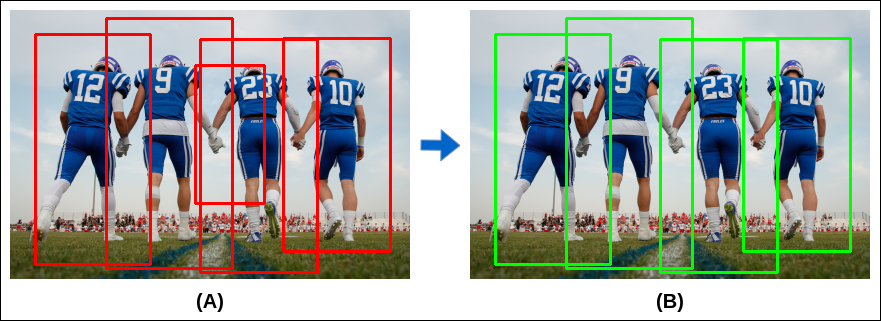
\includegraphics{6-Desenvolvimento-Projeto/imagens-desenvolvimento/comparativo_imagem.png}}
	\end{center}
	\centering \legend{Fonte: Elaborada pelos autores.}
\end{figure}